\documentclass{beamer}

\usetheme{polimi}

\usepackage{colortbl}
\usepackage{longtable}

\title{Students\&Companies}
\subtitle{Requirements and Design Documents}
\author{Andrea Carrara and Federica Currò Dossi}
\date{February 7, 2025}

\begin{document}

\begin{frame}
    \maketitle
\end{frame}

\begin{frame}{Goals}
\newcounter{g}
\setcounter{g}{1}
\newcommand{\gc}{\theg\stepcounter{g}}
\renewcommand{\arraystretch}{1.5}
\begin{longtable}{|c|p{8cm}|}
    \hline \rowcolor{polimiblue!40}
    \textbf{ID} & \textbf{Description} \\ \hline
    G\gc & S\&C allows USs to search and apply for POs. \\ \hline
    G\gc & S\&C recommends POs to USs and USs to COs. \\ \hline
    G\gc & S\&C provides support for the selection process. \\ \hline
    G\gc & S\&C allows USs, COs and UNs to monitor INs. \\ \hline
    G\gc & S\&C collects feedback from USs and COs. \\ \hline
\end{longtable}
\end{frame}

\begin{frame}{Phenomena}
\renewcommand{\arraystretch}{1.5}
\begin{longtable}{|c|p{8cm}|}
    \hline \rowcolor{polimiblue!40}
    \textbf{ID} & \textbf{Description} \\ \hline
    ... & ... \\ \hline
    SP14 & A US accepts a recommended PO. \\ \hline
    SP15 & A US declines a recommended PO. \\ \hline
    ... & ... \\ \hline
    SP37 & A CO accepts a recommended US. \\ \hline
    SP38 & A CO declines a recommended US. \\ \hline
    ... & ... \\ \hline
\end{longtable}
\end{frame}

\begin{frame}{Requirements}
\renewcommand{\arraystretch}{1.5}
\begin{longtable}{|c|p{8cm}|}
    \hline \rowcolor{polimiblue!40}
    \textbf{ID} & \textbf{Description} \\ \hline
    ... & ... \\ \hline
    R14 & S\&C allows USs to accept a recommended PO. \\ \hline
    R15 & S\&C allows USs to decline a recommended PO. \\ \hline
    ... & ... \\ \hline
    R37 & S\&C allows COs to accept a recommended US. \\ \hline
    R38 & S\&C allows COs to decline a recommended US. \\ \hline
    ... & ... \\ \hline
\end{longtable}
\end{frame}

\begin{frame}{State Diagram}
\begin{figure}
    \centering
    \includegraphics[width=11.5cm]{images/state-diagram.png}
\end{figure}
\end{frame}

\begin{frame}{Sequence Diagram}
\begin{figure}
    \centering
    \includegraphics[width=5.5cm]{images/sequence-diagram-1.png}
\end{figure}
\end{frame}

\begin{frame}{Formal Analysis}
\begin{figure}
    \centering
    \includegraphics[width=8.5cm]{images/formal-analysis.png}
\end{figure}
\end{frame}

\begin{frame}{Class Diagram}
\begin{figure}
    \centering
    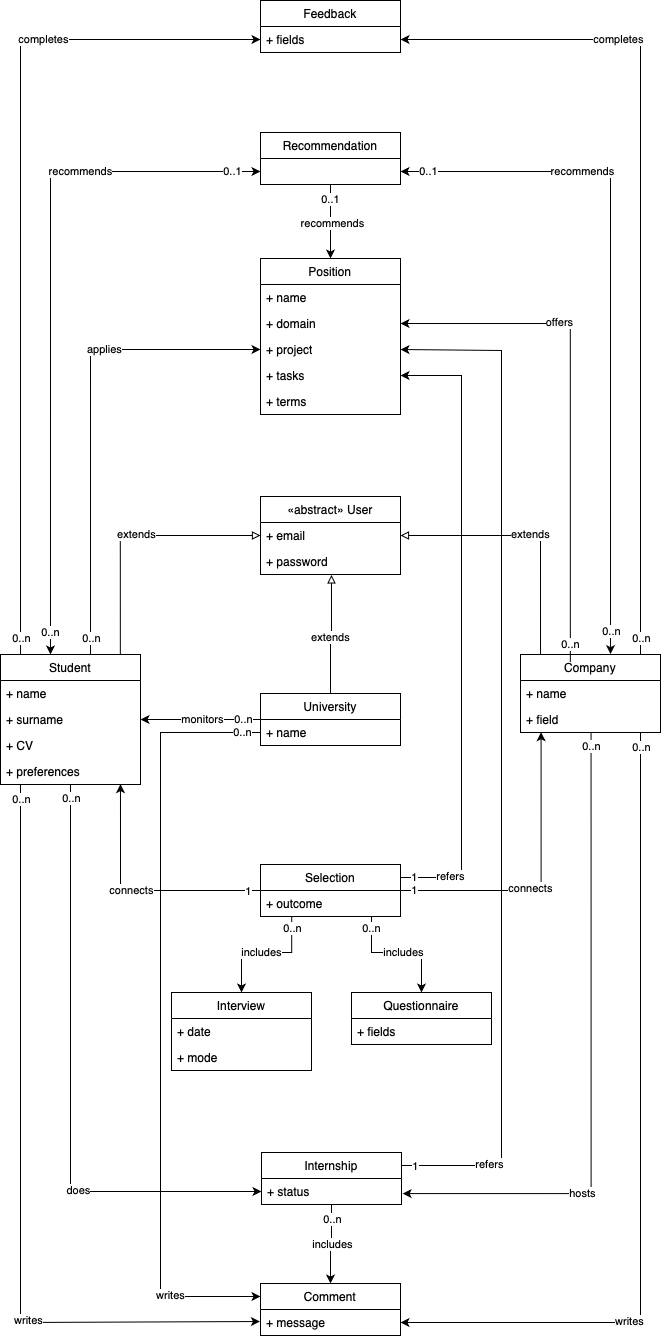
\includegraphics[width=3cm]{images/class-diagram.png}
\end{figure}
\end{frame}

\begin{frame}{Architecture Overview}
\begin{figure}
    \centering
    \includegraphics[width=6cm]{images/architecture-overview.png}
\end{figure}
\end{frame}

\begin{frame}{Deployment View}
\begin{figure}
    \centering
    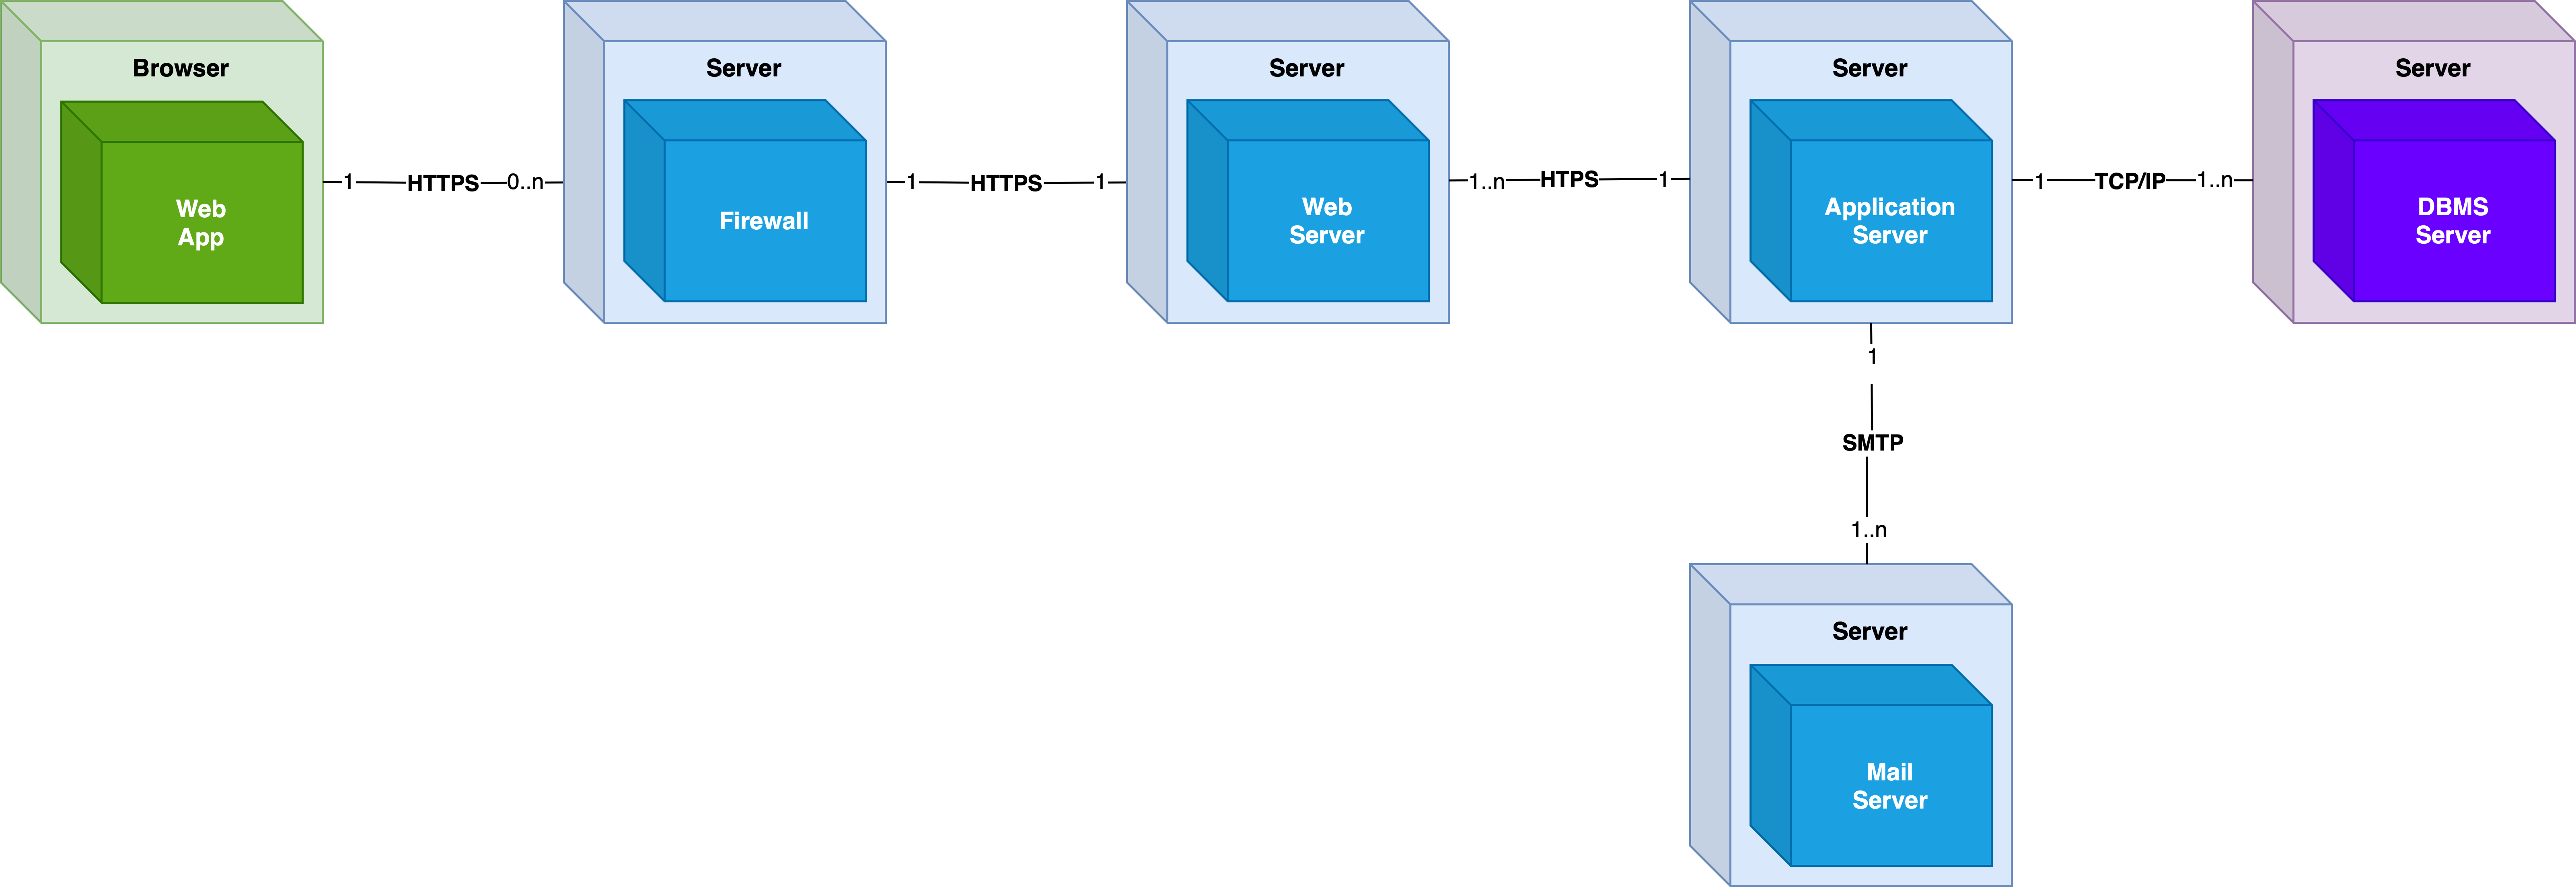
\includegraphics[width=11.5cm]{images/deployment-view.png}
\end{figure}
\end{frame}

\begin{frame}{Component View}
\begin{figure}
    \centering
    \includegraphics[width=11.5cm]{images/component-view.png}
\end{figure}
\end{frame}

\begin{frame}{Managers}
\begin{figure}
    \centering
    \includegraphics[width=11.5cm]{images/managers.png}
\end{figure}
\end{frame}

\begin{frame}{Submanagers}
\begin{figure}
    \centering
    \includegraphics[width=11.5cm]{images/manager.png}
\end{figure}
\end{frame}

\begin{frame}{Sequence Diagram}
\begin{figure}
    \centering
    \includegraphics[width=7cm]{images/sequence-diagram-2.png}
\end{figure}
\end{frame}

\begin{frame}{User Interface Design}
\begin{figure}
    \centering
    \includegraphics[width=4.5cm]{images/user-interface-design.png}
\end{figure}
\end{frame}

\begin{frame}{Wireframe}
\begin{figure}
    \centering
    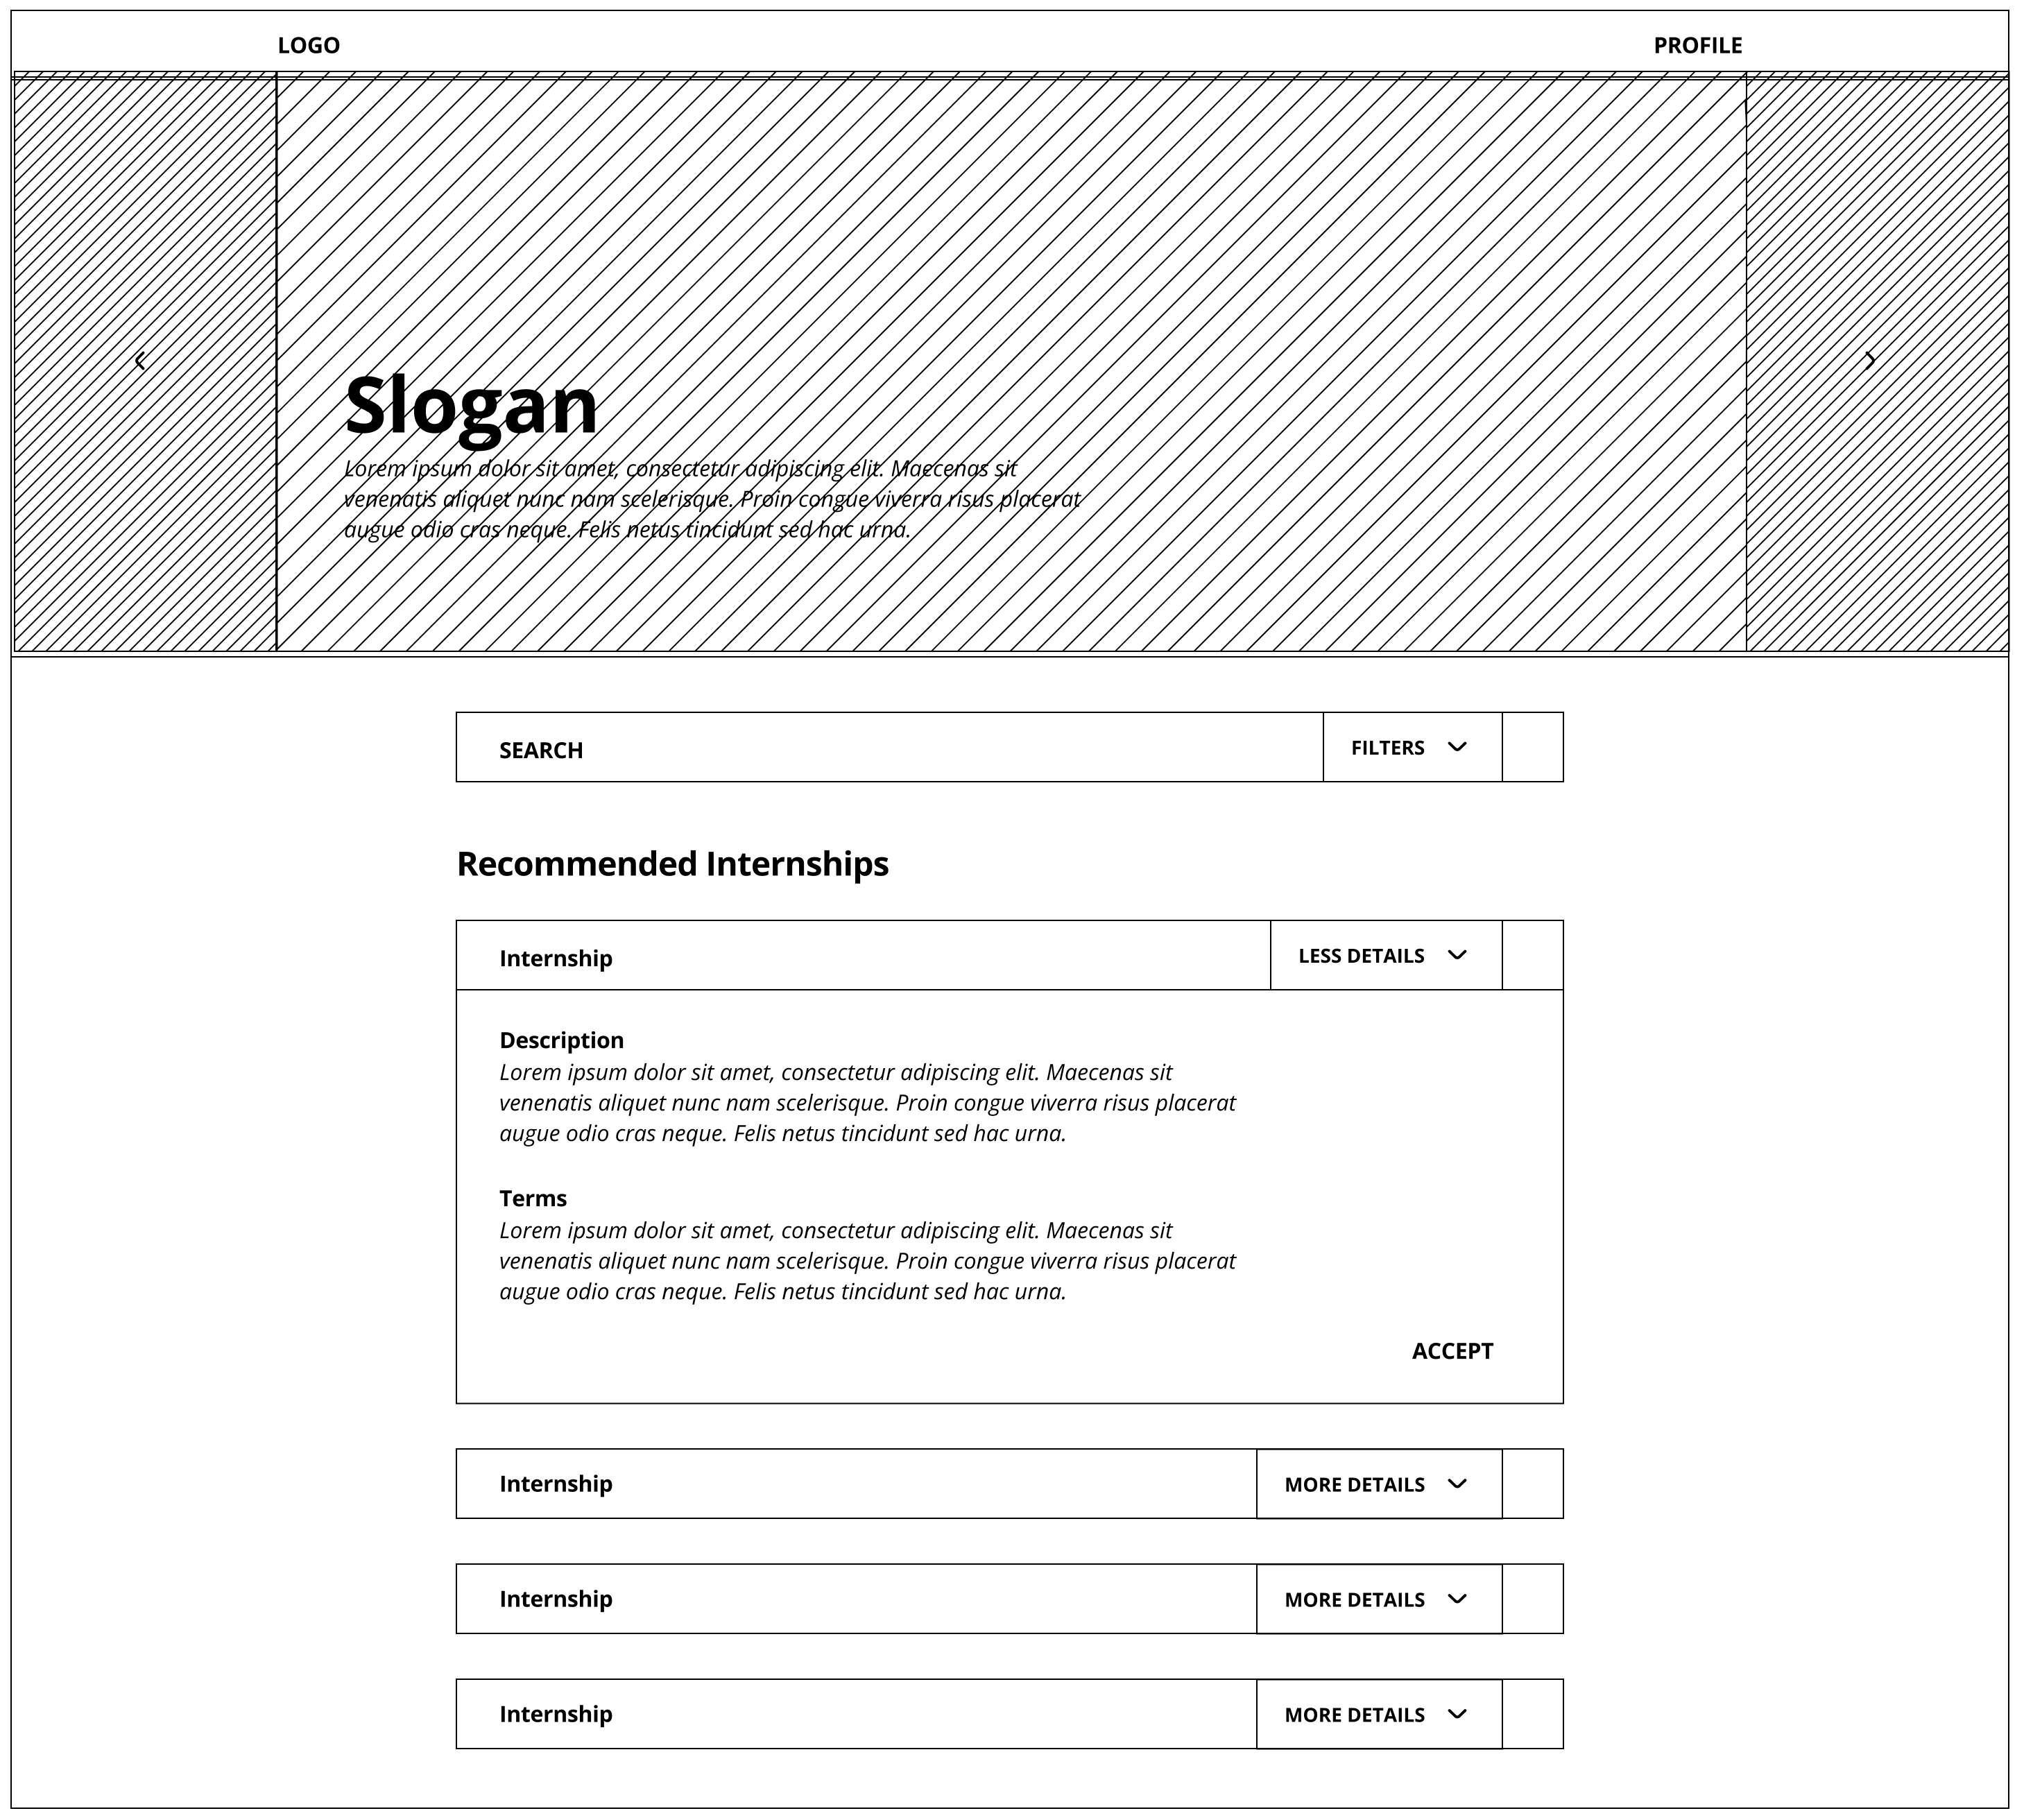
\includegraphics[width=7cm]{images/wireframe.png}
\end{figure}
\end{frame}

\begin{frame}{Conclusion}
\centering \huge
Questions?
\end{frame}

\end{document}
